\section{Scheduling} \label{sc:scheduling}
In scheduling the aim is to meet all hard deadlines and handle soft deadlines of jobs in the best possible manner and avoid deadlocks while doing so. The arrival time of a job is the moment in time it arrives at a processor, while the
release time of a job is the moment in time it becomes available for execution. A task can have different job types and such as perodic, sporadic and Aperiodic. A task is a set of jobs known at the start of the system or triggered by a external event.
A periodic task is defined by three parameters:
\begin{itemize}
	\itemsep0em
	\item The release time r of the first periodic job.
	\item The period p, which is a periodic time interval, at the start of which a periodic job is released.
	\item The execution time e of each periodic job.
	\item The deadline d of each periodic job.
\end{itemize}
and is written as (\textit{r},\textit{p},\textit{e},\textit{d})

\subsection{Rate-monotonic scheduler}
The rate-monotonic scheduling strategy gives a higher priority, to periodic jobs with a shorter period. Because of the static nature of the scheduler, it is easy to compute and predict.\footnote{\cite{Fokkink1965} p.183}


--- This can be removed if we need space?
We define three periodic jobs; $J_1$ with a period of 20 and a execution time of 3, $J_2$ with a period of 5 and a execution time of 2, $J_1$ with a period of 10 and a execution time of 2. All with a release time of 0. on Figure \ref{fig:rateMonotonicExample} we see the outcome using a rate-monotonic scheduler.
---

\begin{figure}[h!]\label{}
	\centering
	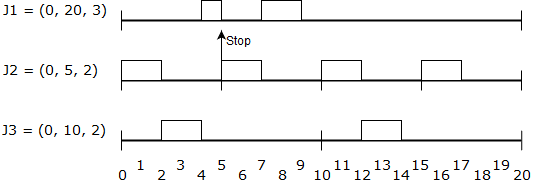
\includegraphics[scale=0.5]{realTimeComputing/fig/rate-mono.png}
	\caption{Example of rate-monotonic scheduling.}
	\label{fig:rateMonotonicExample}
\end{figure}

As we can see on Figure \ref{fig:rateMonotonicExample}, the first job to be executed is $J_2$ followed by $J_3$. $J_1$ is then started but gets preempted by the scheduler, because $J_2$ starts a new execution on period 5. $J_2$ has a shorter period and therefore has a higher priority. $J_3$ continues execution after $J_1$.

\subsection{Earliest deadline first scheduler}
This scheduling strategy will give a higher priority to jobs if its deadline is
earlier. In case of preemptive jobs and no competition for resources, this scheduler
is optimal, in the sense that if utilization at a processor does not exceed one, then
periodic jobs will be scheduled in such a way that no deadlines are missed.\footnote{\cite{Fokkink1965} p.184}

The example in Figure \ref{fig:EarliestDeadlineFirstAndLeastSlacktimeFirstSchedulerExample}, can be viewed as using Earliest deadline first scheduler. The first job to be executed is $J_2$ because it has earliest deadline followed by $J_1$ and $J_3$.

\subsection{Least-slacktime-first scheduler}
This scheduling strategy gives higher priority to jobs wit less slack (Idle time). This scheduler is a good choice if utilization at a processor does not exceed one. In this case the periodic jobs will be scheduled in such a way that no deadlines are missed.\footnote{\cite{Fokkink1965} p.184}

The example in Figure \ref{fig:EarliestDeadlineFirstAndLeastSlacktimeFirstSchedulerExample}, can be viewed as using Least-slacktime-first scheduler. The first job to be executed is $J_2$ because it has the least slacktime followed by $J_1$ and $J_3$.

\begin{figure}[h!]\label{}
	\centering
	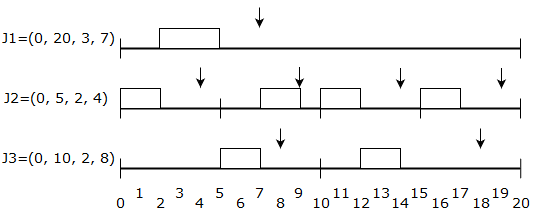
\includegraphics[scale=0.5]{realTimeComputing/fig/EarliestDeadlineFirst.png}
	\caption{Example of Earliest deadline first or Least-slacktime-first scheduler.}
	\label{fig:EarliestDeadlineFirstAndLeastSlacktimeFirstSchedulerExample}
\end{figure}

\subsection{Resource control}
Write about resource control/deadlock
Priority inheirtance
Priority ceiling
Find Søren Hansen (grandmaster) drawings/references